%! Author = spruhs
%! Date = 25.02.25

% Preamble
\documentclass[11pt]{article}

% Packages
\usepackage[utf8]{inputenc}
\usepackage[T1]{fontenc}
\usepackage[ngerman]{babel}
\usepackage{graphicx}
\usepackage{tcolorbox}
\usepackage{tocloft}
\usepackage{appendix}
\usepackage{csquotes}
\usepackage[
    backend=biber,
    style=alphabetic,
]{biblatex}
\usepackage{color}
\usepackage{listings}
\usepackage{xcolor}
\addbibresource{literaturverzeichnis.bib}


% Farben für Syntax-Highlighting definieren
\definecolor{codegreen}{rgb}{0,0.6,0}
\definecolor{codegray}{rgb}{0.5,0.5,0.5}
\definecolor{codepurple}{rgb}{0.58,0,0.82}
\definecolor{backcolour}{rgb}{0.95,0.95,0.92}

% Kotlin-Sprache für listings konfigurieren
\lstdefinelanguage{Kotlin}{
    morekeywords={fun, class, object, val, var, when, if, else, for, while, return, import, package, is, as, null, true, false},
    sensitive=true,
    morecomment=[l]{//},
    morecomment=[s]{/*}{*/},
    morestring=[b]",
}

% Java-Sprache für listings konfigurieren (Java ist bereits vordefiniert, aber hier ein Beispiel für Anpassungen)
\lstdefinelanguage{Java}{
    morekeywords={public, private, protected, class, static, void, if, else, while, for, return, import, package, new},
    sensitive=true,
    morecomment=[l]{//},
    morecomment=[s]{/*}{*/},
    morestring=[b]",
}

\lstset{
    backgroundcolor=\color{backcolour},
    commentstyle=\color{codegreen},
    keywordstyle=\color{codepurple},
    numberstyle=\tiny\color{codegray},
    stringstyle=\color{red},
    basicstyle=\ttfamily\footnotesize,
    breakatwhitespace=false,
    breaklines=true,
    captionpos=b,
    keepspaces=true,
    numbers=left,
    numbersep=5pt,
    showspaces=false,
    showstringspaces=false,
    showtabs=false,
    tabsize=2
}

% Document
\begin{document}

    \begin{titlepage}
        \centering
        {\scshape\LARGE Seminar 1908 Moderne Programmiertechniken und -Methoden -Sommer 2025 \par}
        \vspace{1cm}
        {\huge\bfseries Kotlin statt Java\par}
        \vspace{1.5cm}
        {\scshape\Large Fabian Spruhs\par}
        {\scshape fabian@spruhs.com\par}
        \vspace{2cm}
        {\Large\itshape Studiengang Bachelor Informatik\par}
        \vspace{2cm}


        {\large \today\par}
    \end{titlepage}

    \tableofcontents
    \newpage


    \section{Einleitung}


    \section{Kurzvorstellung Java}

    \subsection{Übersicht}
    \begin{itemize}
        \item \textbf{Erscheinungsjahr:} 1995
        \item \textbf{Entwickler:} Sun Microsystems
        \item \textbf{Entwickler ab 2009:} Oracle Corporation
        \item \textbf{Programier paradigmen:} objektorientiert
        \item \textbf{Aktuelle LTS version:} 21
    \end{itemize}

    \subsection{Technischer Hintergrund}
    Java ist eine Programmiersprache, die von Sun Microsystems entwickelt und im Jahr 1995 veröffentlicht wurde.
    Sie zeichnet sich durch ihre Plattformunabhängigkeit, hohe Robustheit und vielseitigen Einsatzmöglichkeiten aus,
    wodurch sie insbesondere in der Industrie und im Unternehmensumfeld eine zentrale Rolle spielt.

    Ein wesentliches Merkmal von Java ist die Art der Code-Ausführung.
    Anstatt direkt in Maschinencode übersetzt zu werden, wird der Quellcode zunächst in Bytecode kompiliert.
    Dieser Bytecode wird anschließend von der Java Virtual Machine (JVM) interpretiert und ausgeführt.
    Durch dieses Konzept ist Java nicht an eine spezifische Prozessorarchitektur oder ein
    bestimmtes Betriebssystem gebunden, was eine hohe Portabilität gewährleistet.
    Diese Plattformunabhängigkeit stellt einen bedeutenden Vorteil dar, den
    viele andere Programmiersprachen im Laufe der Zeit übernommen haben.

    Neben der Plattformunabhängigkeit bietet die JVM zahlreiche zusätzliche
    Funktionen, die zur Stabilität und Sicherheit von Java-Anwendungen beitragen.
    Dazu gehören unter anderem eine automatische Speicherverwaltung
    durch den Garbage Collector, eine starke Typisierung zur Minimierung
    von Laufzeitfehlern sowie eine integrierte Unterstützung für Multithreading,
    die eine effiziente nebenläufige Verarbeitung ermöglicht. \cite[51 - 54]{insel}

    Java basiert konsequent auf dem objektorientierten Programmierparadigma, das die Strukturierung von Software in Klassen und Objekte ermöglicht. \\

    \subsection{Verbreitung}
    Der TIOBE-Index misst monatlich die Popularität und Verbreitung von Programmiersprachen~\cite{tiobe}.
    Laut diesem Index zählt Java zu den am weitesten verbreiteten Programmiersprachen weltweit.
    Wie in Abbildung~\ref{fig:entwicklung-tiobe} ersichtlich, befand sich Java über fast zwei Jahrzehnte hinweg
    kontinuierlich unter den Top 3 der relevantesten Programmiersprachen.

    In den letzten Jahren hat die Popularität von Java zwar leicht nachgelassen, dennoch bleibt die Sprache weiterhin
    von großer Bedeutung.
    Auch im Februar 2025 belegte Java den dritten Platz im TIOBE-Index
    (siehe Abbildung~\ref{fig:tiobe-java-2025}).

    Java ist die Basis zahlreicher Anwendungen und wird in vielfältigen Bereichen eingesetzt.
    Darüber hinaus
    verfügt Java über eine umfangreiche Ökosystemlandschaft mit einer Vielzahl an Bibliotheken, Paketen,
    Frameworks und Fachliteratur.

    Die weltweite Java-Community ist äußerst aktiv und umfasst eine große Anzahl an erfahrenen Entwicklern,
    die kontinuierlich zum Wissenstransfer und zur Weiterentwicklung der Sprache beitragen.
    Ein Beispiel für die Größe dieser Infrastruktur ist das Maven-Repository, das über 2.800 Repositories mit mehr als 52 Millionen Java-Paketen
    enthält~\cite{maven}.

    Diese etablierte und breit aufgestellte Infrastruktur stellt einen weiteren entscheidenden Vorteil von Java dar und
    trägt zu seiner anhaltenden Relevanz in der Softwareentwicklung bei.\\


    \section{Kurzvorstellung kotlin}

    \subsection{Übersicht}
    \begin{itemize}
        \item \textbf{Erscheinungsjahr:} 2011
        \item \textbf{Entwickler:} Jetbrains
        \item \textbf{Programier paradigmen:} objektorientiert, funktional
        \item \textbf{Aktuelle LTS version:} 2.1.0
    \end{itemize}

    \subsection{Technischer Hintergrund}
    Kotlin wurde 2011 von der Firma JetBrains veröffentlicht.
    Ziel der Entwicklung war es, eine verbesserte Alternative zu Java zu schaffen.
    Schon an der Namensgebung kann man die nähe zu Java erkennen.
    Der Name Java bezieht sich auf eine Indonesiche Insel.
    Der Namensgeber von Kotlin ist eine russische Insel vor St. Petersburg.

    Obwohl Java nur etwa 15 Jahre älter als Kotlin ist, stellt dies in der schnelllebigen Welt der Softwareentwicklung eine erhebliche Zeitspanne dar.
    In vielerlei Hinsicht wirkt Java inzwischen veraltet.
    Die Syntax ist vergleichsweise umständlich, und einige moderne Sprachfeatures, die in anderen Programmiersprachen standardmäßig verfügbar sind, fehlen in Java oder
    müssen umständlich über externe Tools nachgerüstet werden.
    Zudem setzt Java ausschließlich auf das objektorientierte Paradigma,
    während moderne Programmiersprachen häufig eine Kombination aus objektorientierter und funktionaler Programmierung unterstützen.

    Bei der Entwicklung von Kotlin hat JetBrains bewusst aus den Designfehlern von Java gelernt.
    Gleichzeitig wurden essenzielle Eigenschaften, die zur Popularität von Java beigetragen haben, beibehalten.

    Kotlin-Code wird ebenfalls in Bytecode kompiliert und kann auf der Java Virtual Machine (JVM) ausgeführt werden.
    Dies bietet den großen Vorteil, dass Kotlin-Programme überall dort lauffähig sind, wo auch Java-Code ausgeführt werden kann.
    Zudem kann Kotlin auf sämtliche vorhandenen Java-Bibliotheken zugreifen und diese nutzen, wodurch nahezu das gesamte Java-Ökosystem zur Verfügung steht.
    Die Interoperabilität zwischen Kotlin und Java geht sogar noch weiter.
    Beide Sprachen lassen sich nahtlos in einem Projekt kombinieren.
    Dadurch können auch bestehende Java-Anwendungen schrittweise mit Kotlin weiterentwickelt werden~\cite[19-20]{kotlin-handbuch}.

    \subsection{Verbreitung}
    Nach dem TIOBE index befindet sich Kotlin im März 2025 nur auf Platz 19 der relevantesten Sprachen, siehe Abbildung~\ref{fig:tiobe-kotlin-2025}.
    Es gibt aber auch gute Nachrichten für Kotlin im Bezug auf die Verbreitung und relevanz.
    Kotlin wurde von Google zu der bevorzugten Sprache für die Android Entwicklung erklärt~\cite{tn3-google}.

    \section{Interoperabilität zwischen Java und Kotlin}

    \subsection{Kotlin in Java integrieren}
    Kotlin und Java lassen sich problemlos in einem Projekt kombinieren, was mehrere Vorteile mit sich bringt.
    Einerseits können in Kotlin geschriebene Pakete in Java verwendet werden und umgekehrt.
    Andererseits ermöglicht diese Kompatibilität, bestehende Java-Projekte mit Kotlin weiterzuführen oder
    schrittweise auf Kotlin umzustellen, ohne den vorhandenen Code sofort ersetzen zu müssen.
    Dies ist besonders relevant für Unternehmen mit großen Java-Codebasen, die nicht abrupt auf Kotlin wechseln können. \cite[20]{kotlin-handbuch}

    Im folgenden Beispiel werden verschiedene Möglichkeiten vorgestellt, wie Kotlin-Code in einer Java-Umgebung ausgeführt
    werden kann. Die zugehörige \texttt{.java}-Datei enthält eine Java-Klasse mit einer \texttt{main}-Methode.
    In dieser Datei wird Kotlin-Code aus einer \texttt{.kt}-Datei importiert und ausgeführt, da Kotlin-Quellcode stets
    in Dateien mit der Endung \texttt{.kt} gespeichert wird.

    \begin{lstlisting}[language=Kotlin, caption={KotlinGreeter.kt}]
package main.java.com.spruhs

class ClassGreeter {
    fun greet() {
        println("Hello from kotlin class method!")
    }
}

class StaticGreeter {
    companion object {

        @JvmStatic
        fun greet() {
            println("Hello from kotlin static method!")
        }
    }
}

object SingletonGreeter {
    fun greet() {
        println("Hello from kotlin singleton method!")
    }
}
    \end{lstlisting}

    \begin{lstlisting}[language=Java, caption={Main.java}]
import main.java.com.spruhs.ClassGreeter;
import main.java.com.spruhs.SingletonGreeter;
import main.java.com.spruhs.StaticGreeter;

public static void main(String[] args) {
    ClassGreeter classGreeter = new ClassGreeter();
    classGreeter.greet();

    StaticGreeter.greet();

    SingletonGreeter.INSTANCE.greet();
}
    \end{lstlisting}

    \begin{tcolorbox}[colback=black!5!white, colframe=black, title=Ausgabe]
        Hello from kotlin class method!\\
        Hello from kotlin static method!\\
        Hello from kotlin singleton method!
    \end{tcolorbox}
    
    \subsection{Java in Kotlin integrieren}
    Auch umgekehrt ist die Integration von Java in Kotlin möglich. Dies hat vor allem den Vorteil, dass bestehende Java-Bibliotheken und -Frameworks
    in Kotlin-Projekten verwendet werden können. Im folgenden Beispiel werden 2 verschiedene Möglichkeiten vorgestellt, wie Java-Code von Kotlin importiert und ausgeführt wird.

    \begin{lstlisting}[language=Java, caption={JavaClassMethodGreeter.java}]
package main.kotlin.com.spruhs;

public class JavaClassMethodGreeter {
    public void greet() {
        System.out.println("Hello from java class method!");
    }
}
    \end{lstlisting}

    \begin{lstlisting}[language=Java, caption={JavaStaticGreeter.java}]
package main.kotlin.com.spruhs;

public class JavaStaticGreeter {
    public static void greet() {
        System.out.println("Hello from java static method!");
    }
}

    \end{lstlisting}

    \begin{lstlisting}[language=Kotlin, caption={Main.kt}]
package main.kotlin.com.spruhs

fun main() {
    val javaClassMethodGreeter = JavaClassMethodGreeter()
    javaClassMethodGreeter.greet()

    JavaStaticGreeter.greet()
}
    \end{lstlisting}

    \begin{tcolorbox}[colback=black!5!white, colframe=black, title=Ausgabe]
        Hello from java class method!\\
        Hello from java static method!\\
    \end{tcolorbox}

    \section{Features}

    \subsection{Kurzübersicht}

    In der folgenden Tabelle~\ref{tab:kotlin-java-features} werden die Features die Kotlin von Java unterscheiden kurz vorgestellt. Danach werden die
    wichtigsten Features genauer erläutert. \\
    Bei den Features die Java hat aber Kotlin nicht gibt es einige die komplett wegfalle und einige die in Kotlin durch andere Features ersetzt wurden.
    Anstelle von Static-members gibt es in Kotlin Companion-Objects. Wildecards werden ersetzt durch declaration-site variance und type projections.
    If abfragen sind in Kotlin Ausdrücke und können so den Ternary-Operator ersetzen. Das Pattern-Matching wird in Kotlin durch die Smart-Casts ersetzt.
    Die records als einfacher Datencontainer wurde in Kotlin durch die data class ersetzt.\\
    Die Checked Exceptions gibt es in Kotlin nicht mehr. Auch die Package private visibility modifier wurde in Kotlin entfernt.
    Die Primitiven Datentypen wurden in Kotlin durch die Wrapper-Klassen ersetzt. Allerdings werden die primitiven Datentypen noch im byte-code verwendet.\\
    \cite{doc-comparison}

    \begin{table}[h!]
        \centering
        \begin{tabular}{|c|c|}
            \hline
            \textbf{Kotlin-Features, die Java nicht hat} & \textbf{Java-Features, die Kotlin nicht hat} \\
            \hline
            \hline
            Lambda expressions & Checked Exceptions \\
            \hline
            Inline functions & Primitive types \\
            \hline
            Extension functions & Wildcard-types \\
            \hline
            Null-safety & Ternary-Operator \\
            \hline
            Default properties & Records \\
            \hline
            Smart casts & Static members \\
            \hline
            Primary constructors & Pattern Matching \\
            \hline
            First-class delegation & package-private visibility modifier \\
            \hline
            Declaration-site variance and Type projections &  \\
            \hline
            Singletons &  \\
            \hline
            Range expressions &  \\
            \hline
            Operator overloading &  \\
            \hline
            Companion objects &  \\
            \hline
            Data classes &  \\
            \hline
            Coroutines &  \\
            \hline
            Top-level functions &  \\
            \hline
            Default arguments &  \\
            \hline
            Named parameters &  \\
            \hline
            Infix functions &  \\
            \hline
            Expect and actual declarations &  \\
            \hline
            Explicit API Mode and better control of API surface &  \\
            \hline
        \end{tabular}
        \caption{Vergleich Kotlin und Java Features}
        \label{tab:kotlin-java-features}
    \end{table}

    \subsection{Null-safety}
    Tony Hoare war 1965 an der Einführung der ersten Null-Referenz in der Objektorientierte Sprache ALGOL W beteiligt.
    Im Jahre 2009 bezeichnete er dies als "Milliarden-Dollar-Fehler"~\cite{billion-dollar-mistake}.
    In Java wurde dieser Fehler durch die Einführung von \texttt{null} als Referenzwert weitergeführt.
    Dort können alle Referenztypen, ausser den Primitiven Datentypen, den Wert \texttt{null} annehmen.
    Dies führt zu einer Vielzahl von NullPointerExceptions, die in Java-Programmen auftreten können.
    Um dies zu verhindern müsste man in Java jedes mal überprüfen ob eine Referenz \texttt{null} ist bevor man auf diese zugreift.
    Wenn man das im Code Konsequenz umsetzten würde, wird dass zu sehr viel Boilerplate Code führen der die Lesbarkeit des Codes verschlechtert.\\
    Kotlin hat aus diesem Fehler gelernt und setzt auf Null-Safety.
    In Kotlin sind Referenzen standardmäßig nicht nullbar.
    Sie können nur null sein, wenn sie explizit als nullable deklariert werden.
    Dies geschieht durch die Verwendung des Fragezeichens \texttt{?} nach dem Typ.
    Der Compiler erzwingt die Überprüfung von null-Werten und verhindert so das Auftreten von NullPointerExceptions.
    Dieses Feature trägt erheblich zur Robustheit und Stabilität von Kotlin-Programmen bei und erleichtert die Fehlersuche und -behebung.
    In Listing \ref{lst:kotlin-null-safety} wird die Null-Safety in Kotlin demonstriert.
    Es werden zuerst zwei Variabeln vom Type String deklariert.
    Eine davon ist nullable und die andere nicht.
    Danach werden beiden Vraibeln der Wert \texttt{null} zugewiesen.
    Dies führt bei der nicht nullable Variabel zu einem Compiler Fehler. \\

    Weiterhin bietet Kotlin noch möglichkeiten mit null-Werten umzugehen.
    Dazu gibt es zum einem die Möglichkeit mit dem Operator \texttt{?.} auf eine Referenz zuzugreifen die potenziell \texttt{null} sein kann.
    Falls diese Referenz \texttt{null} ist wird der Ausdruck nicht weiter ausgeführt und es wird \texttt{null} zurückgegeben und keine NullPointerException ausgelöst.
    Weiterhin gibt es den Elvis-Operator \texttt{?:} der es ermöglicht einen Default-Wert zurückzugeben falls die Referenz \texttt{null} ist.
    In Listing~\ref{lst:kotlin-user-null-safety} wird die Null-Safety in Kotlin demonstriert.
    Hierfür gibt es die \texttt{data class} KotlinUser die ein Attribut \texttt{name} hat.
    Die Funktion nimmt ein KotlinUser Objekt entgegen das Potenziell \texttt{null} sein kann und gibt den Namen zurück.
    Durch den \texttt{?.} Operator kann auf das Attribut \texttt{name} zugegriffen werden ohne vorher zu überprüfen ob das Objekt \texttt{null} ist.
    Falls das Objekt \texttt{null} ist wird durch den \texttt{?:} Operator der Default-Wert \texttt{Unbekannter Benutzer} zurückgegeben.
    Dies wird in der Main Methode einmal mit einem Objekt und einmal mit einem \texttt{null} Wert demonstriert.\\
    In Listing~\ref{lst:java-user-null-safety} wird das gleiche Beispiel in Java gezeigt.
    Hier lässt sich gut ablesen wie viel Boilerplate Code in Java notwendig ist um das gleiche Ergebnis zu erzielen.




    \begin{lstlisting}[language=Kotlin, caption={KotlinNullSafety.kt}, label={lst:kotlin-null-safety}]
    fun testNullSafety() {
        var nullableVariable: String?
        var nonNullableVariable: String

        nullableVariable = null // Kein Compiler Fehler
        nonNullableVariable = null // Compiler Fehler
    }
    \end{lstlisting}

    \begin{lstlisting}[language=Kotlin, caption={KotlinUser.kt}, label={lst:kotlin-user-null-safety}]
        package main.kotlin.com.spruhs

        fun getUserName(user: KotlinUser?): String {
        return user?.name ?: "Unbekannter Benutzer"
        }

        data class KotlinUser(val name: String)

        fun main() {
        val user1: KotlinUser = KotlinUser("Fabian")
        val user2: KotlinUser? = null

        println(getUserName(user1)) // Ausgabe: Fabian
        println(getUserName(user2)) // Ausgabe: Unbekannter Benutzer
        }
    \end{lstlisting}

    \begin{lstlisting}[language=Java, caption={NullHandlingExample.java}, label={lst:java-user-null-safety}]
    package main.kotlin.com.spruhs;

class JavaUser {
    private String name;

    public JavaUser(String name) {
        this.name = name;
    }

    public String getName() {
        return name;
    }
}

public class NullHandlingExample {
    public static String getUserName(JavaUser user) {
        return (user != null && user.getName() != null) ? user.getName() : "Unbekannter Benutzer";
    }

    public static void main(String[] args) {
        JavaUser user1 = new JavaUser("Fabian");
        JavaUser user2 = null;

        System.out.println(getUserName(user1)); // Ausgabe: Fabian
        System.out.println(getUserName(user2)); // Ausgabe: Unbekannter Benutzer
    }
}
    \end{lstlisting}

    \subsection{Funktionale Programierung}

    Funktionale Programierung hat in den letzten Jahren mehr an bedeutung gewonnen.
    Ein grund dafür ist, dass entwicklung der CPU Geschwindigkeit nicht mehr so gross ist wie in den vorherigen Jahren.
    Aus diesem Grund ist es wichtig geworden, das Programme paralleler ausgeführt werden.
    So kann die ausführung auf mehrere CPU aufgeteilt werden.
    Die Funktionale Programierung eigenet sich sehr gut um diese Parallelisierung zu erreichen~\cite[129]{kotlin-patterns}.
    Kotlin wurde von anfang an mit dem Ziel entwickelt, eine moderne Programmiersprache zu schaffen, die sowohl objektorientierte als auch funktionale Programmierparadigmen unterstützt.
    Java wurde als rein objektorientierte Sprache entwickelt und hat erst seit der Version 8 funktionale Features hinzugefügt.
    Im folgenden werden einige der wichtigsten funktionalen Features von Kotlin vorgestellt und mit Java vergleichen, soweit diese dort vorhanden sind.\\

    \subsubsection{Higher-Order-Functions}
    Kotlin unterstützt Higher-Order-Functions, die Funktionen als Parameter akzeptieren oder Funktionen zurückgeben können.
    Dabei sind in Kotlin Funktionen First-Class Citizens, was bedeutet, dass sie wie andere Datentypen behandelt werden können.
    In Java können keine Funktionen übergeben werden.
    Für die Funktionale Programierung in Java wird stattdessen die Funktionalität in einer Methode implementiert, sodass die Funktion zu einem Objekt mit einer Methode wird.
    Lambda-Ausdrücke, bzw. Methoden/Konstruktorreferenzen geben eine kompakte Syntax ohne dabei eine extra Klasse mit einer Methode zu schreiben~\cite[820]{insel}.
    In den folgenden zwei Code Beispielen ist eine Funktion implementiert die zwei Zahlen und eine Funktion entgegen nimmt.
    Die entgegengenommene Funktion nimmt zwei Zahlen entgegen und gibt eine Zahl zurück.
    In Listing~\ref{lst:kotlin-higher-order-function} ist diese Funktion in Kotlin und in Listing~\ref{lst:java-higher-order-function} in Java implementiert.
    An der Kotlin implementierung ist zu sehen, dass keine Klasse für die implementierung Notwendig ist.
    In der Java implementierung wird die Methode als statische methode einer Klasse implementiert.
    Weiterhin ist in der Java implementierung die Funktion als Übergabe Parameter nur in Verbindung mit dem Funktionalen Interface BiFunction möglich.
    Diese muss zuerst noch importiert werden.
    In Kotlin ist solch ein Funktionales Interface nicht nötig.

    \begin{lstlisting}[language=Kotlin, caption={HigherOrderKotlin.kt}, label={lst:kotlin-higher-order-function}]
package main.kotlin.com.spruhs

fun operateOnNumbers(a: Int, b: Int, operation: (Int, Int) -> Int): Int {
return operation(a, b)
}

fun main() {
val sum = operateOnNumbers(5, 3) { x, y -> x + y }
println(sum) // Ausgabe 8
}
    \end{lstlisting}

    \begin{lstlisting}[language=Java, caption={HigherOrderJava.java}, label={lst:java-higher-order-function}]
package main.kotlin.com.spruhs;

import java.util.function.BiFunction;

public class HigherOrderJava {

public static int operateOnNumbers(int a, int b, BiFunction<Integer, Integer, Integer> operation) {
return operation.apply(a, b);
}

public static void main(String[] args) {
int sum = operateOnNumbers(5, 3, (x, y) -> x + y);
System.out.println(sum); // Ausgabe 8
}
}
    \end{lstlisting}

    \subsubsection{Inline Functions}
    Kotlin unterstützt Inline-Funktionen, die es ermöglichen, den Overhead von Funktionsaufrufen zu reduzieren.
    Dies ist besonders nützlich in Verbindung mit Higher-Order-Functions, da es die Leistung verbessert und den Code optimiert.
    Ein vergleichbares Feature in Java ist die Verwendung von Lambda-Ausdrücken, die jedoch nicht den gleichen Grad an Optimierung bieten wie Kotlin's Inline-Funktionen.
    Bei einer inline Funktion wird der Code der Funktion an der Stelle des Aufrufs eingefügt, anstatt einen Funktionsaufruf durchzuführen.
    Dadurch wird der Overhead von Funktionsaufrufen reduziert und die Leistung verbessert.
    In Listing~\ref{lst:kotlin-inline-function} ist eine Inline-Funktion in Kotlin implementiert.
    Diese Funktion nimmt einen String und eine Funktion entgegen, die einen String als Parameter akzeptiert und einen String zurückgibt.
    In der Funktion wird die übergebene Funktion auf den übergebenen String angewendet.
    Dabei wird bei dem Aufruf der Funktion die übergebene Funktion inline in den Code eingefügt.
    Dies wird durch das Schlüsselwort \texttt{inline} erreicht~\cite{kotlin-inline}.

    \begin{lstlisting}[language=Kotlin, caption={HigherOrderJava.java}, label={kotlin-inline-function}]
package main.kotlin.com.spruhs

inline fun transformString(input: String, transform: (String) -> String): String {
    return transform(input)
}

fun main() {
    val result = transformString("Hello, World!") { it.uppercase() }
    println(result) // Ausgabe: HELLO, WORLD!
}
    \end{lstlisting}

    \subsection{Threads und Coroutines}
    In Java werden Threads verwendet, um parallele Ausführung zu ermöglichen.
    Ein Java Thread ist eine 1 zu 1 Abbildung auf einen Betriebssystem-Thread~\cite[940]{insel}.
    Das bedeutet, dass jeder Java-Thread direkt mit einem Betriebssystem-Thread verknüpft ist.
    Zu jedem Thread gehört dann ein eigener Stack und ein eigener Speicherbereich.
    Threads sind in Java relativ schwergewichtig und benötigen viel Overhead.
    Dadurch kann Java nur eine begrenzte Anzahl von Threads gleichzeitig ausführen.
    Zu viele Threads würden sonst sehr schnell zu einem Mangel an Systemressourcen führen.
    Dieses Problem lässt sich in Java mit Thread-Pools lösen.
    Ein Thread-Pool ist eine Sammlung von Threads, die wiederverwendet werden können, um Aufgaben auszuführen.
    Dabei ist die Anzahl der Threads im Pool begrenzt.
    Wenn ein Thread im Pool blockiert, dann kann dafür kein neuer Thread in den Pool aufgenommen werden.
    Es können erst wieder neue Threads in den Pool aufgenommen werden, wenn ein Thread abgeschlossen ist und der Pool wieder Platz hat.
    Dies führt zu einer nicht optimalen Auslastung der Systemressourcen.\\
    Kotlin bietet eine Alternative zu Threads in Form von Coroutines.
    Coroutines sind leichtgewichtige Threads, die eine einfachere und effizientere Möglichkeit bieten, parallele und asynchrone Programmierung zu implementieren.
    Coroutines sind nicht an einen bestimmten System Thread gebunden und können auf verschiedenen Threads ausgeführt werden.
    Die Verwaltung der Coroutines erfolgt durch den Kotlin-Compiler, der den Overhead von Funktionsaufrufen und Kontextwechseln optimiert.
    Dabei können Coroutines in einem Thread-Pool ausgeführt werden, ohne dass die Anzahl der Threads im Pool begrenzt ist.
    Wenn eine Coroutine blockiert, wird der aktuelle Thread nicht blockiert.
    Dies ermöglicht eine bessere Auslastung der Systemressourcen und eine höhere Effizienz bei der Ausführung von parallelen Aufgaben~\cite[194]{kotlin-patterns}.
    \\
    Coroutines:\\
    Zeit: 305 ms\\
    Speicher: 2 MB\\
    Counter: 10.000\\

    Thread-Pool 1:\\
    Zeit: 20045 ms\\
    Speicher: 5 MB\\
    Counter: 200\\

    Thread-Pool 10:\\
    Zeit: 20031 ms\\
    Speicher: 4 MB\\
    Counter: 1.995\\

    Thread-Pool 50:\\
    Zeit: 20056 ms\\
    Speicher: 4 MB\\
    Counter: 9.975\\

    Thread-Pool 100:\\
    Zeit: 20073 ms\\
    Speicher: 4 MB\\
    Counter: 10.000\\

    Thread-Pool 500:\\
    Zeit: 20204 ms\\
    Speicher: 5 MB\\
    Counter: 10.000\\

    Thread-Pool 1.000:\\
    Zeit: 20263 ms\\
    Speicher: 4 MB\\
    Counter: 10.000\\

    Thread-Pool 5.000:\\
    Zeit: 21041 ms\\
    Speicher: 5 MB\\
    Counter: 10.000\\

    Thread-Pool 10.000:\\
    Zeit: OutOfMemoryError\\
    Speicher:
    Counter:



    \printbibliography[
        heading=bibintoc,
        title={Literaturverzeichnis}
    ]
    \appendix


    \section{Anhang}

    \begin{figure}[h]
        \centering
        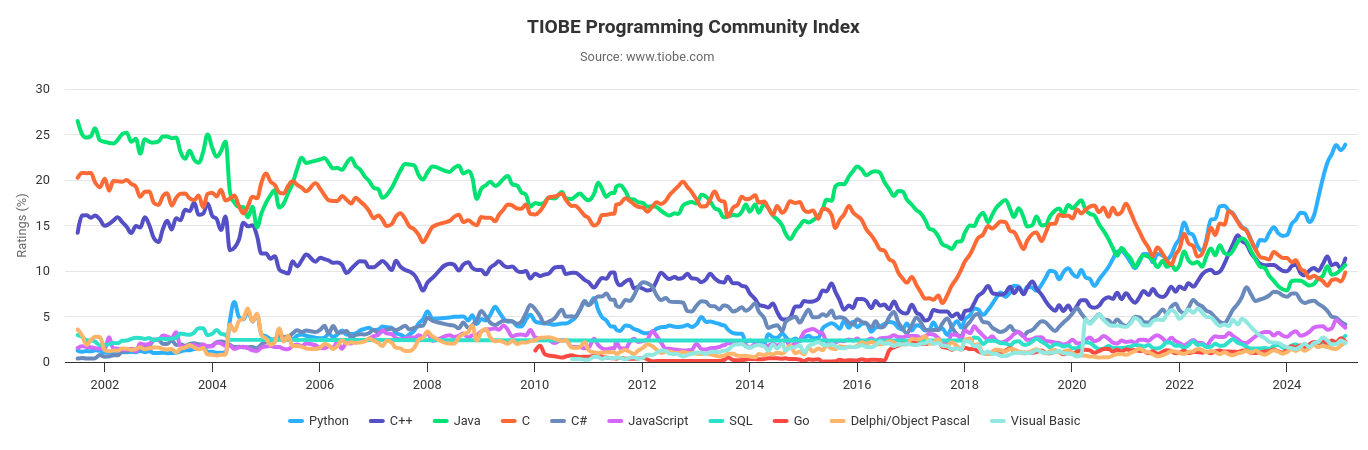
\includegraphics[width=0.8\textwidth]{pictures/Screenshot 2025-02-26 at 19-53-49 TIOBE Index - TIOBE}
        \caption{Entwicklung Tiobe Index 2002 - 2024 vom 26.02.2025 }
        \label{fig:entwicklung-tiobe}
    \end{figure}

    \begin{figure}[h]
        \centering
        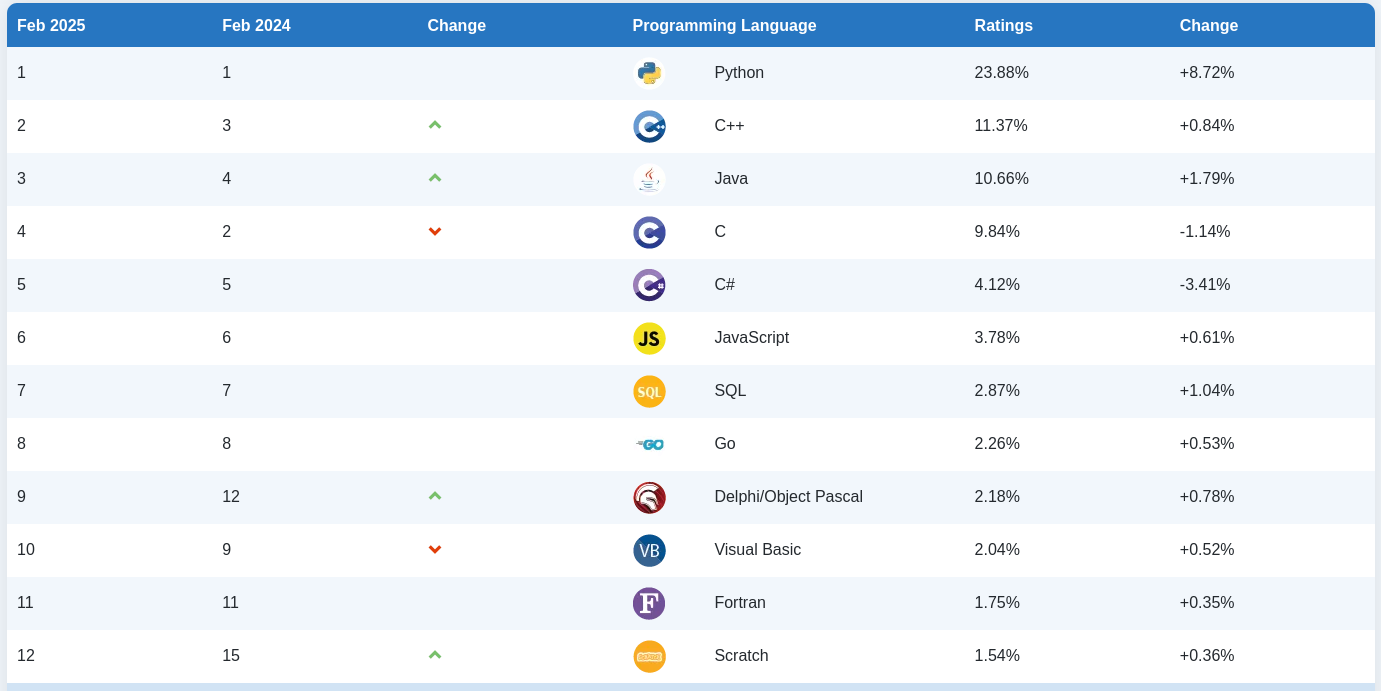
\includegraphics[width=0.8\textwidth]{pictures/Screenshot 2025-02-26 at 19-54-42 TIOBE Index - TIOBE}
        \caption{Tiobe Index Februar 2025 vom 26.02.2025}
        \label{fig:tiobe-java-2025}
    \end{figure}

    \begin{figure}[h]
        \centering
        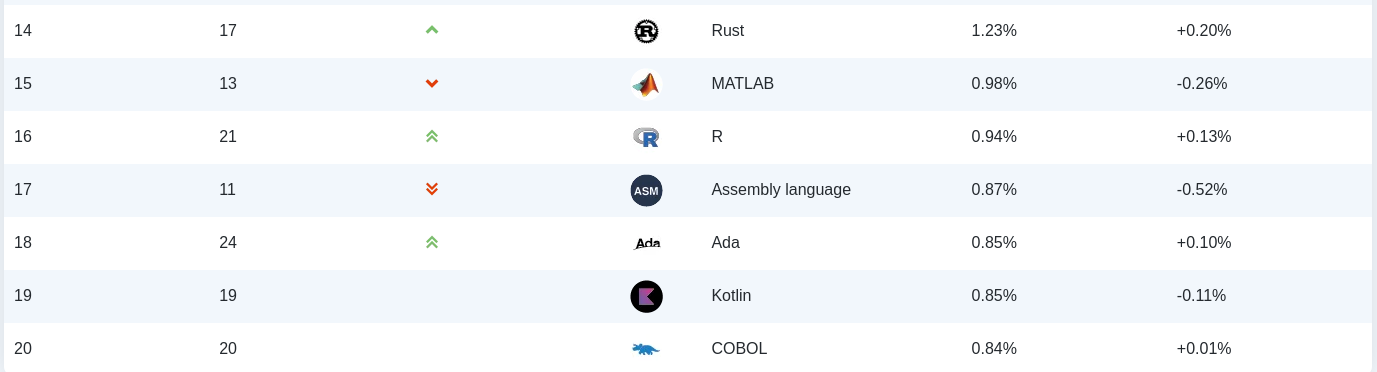
\includegraphics[width=0.8\textwidth]{pictures/Screenshot 2025-03-11 at 22-21-04 TIOBE Index - TIOBE}
        \caption{Tiobe Index März 2025 vom 11.03.2025}
        \label{fig:tiobe-kotlin-2025}
    \end{figure}


\end{document}